\section{Method}
\label{sec:method}
Our system processes multi-camera synchronized video from a 4-corner intersection to reconstruct static and dynamic 3D scene elements for Line-of-Sight visibility analysis. Figure~[3] illustrates the complete pipeline.
% Figure 3: Method pipeline diagram will be inserted here
\subsection{\green{Pass 1: Static Scene Reconstruction}}
\green{We extract static background images per camera via temporal median filtering and apply DUSt3R~\cite{dust3r} for multi-view geometry estimation. DUSt3R jointly optimizes camera poses and produces a dense global point cloud in a shared world frame with consistent camera intrinsics and extrinsics. This provides the geometric foundation for projecting 2D detections to 3D.}
\begin{figure}[h!]
    \centering
    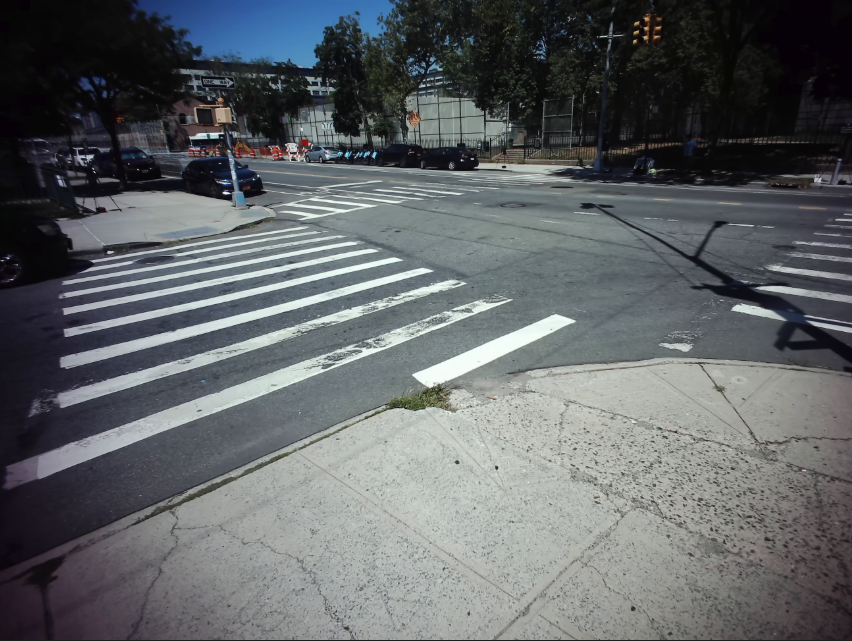
\includegraphics[width=0.8\linewidth]{assets/Static_background.png}
    \caption{Static background without any moving vehicles or pedestrians}
    \label{fig:static_reconstruction}
\end{figure}
\begin{figure}[h!]
    \centering
    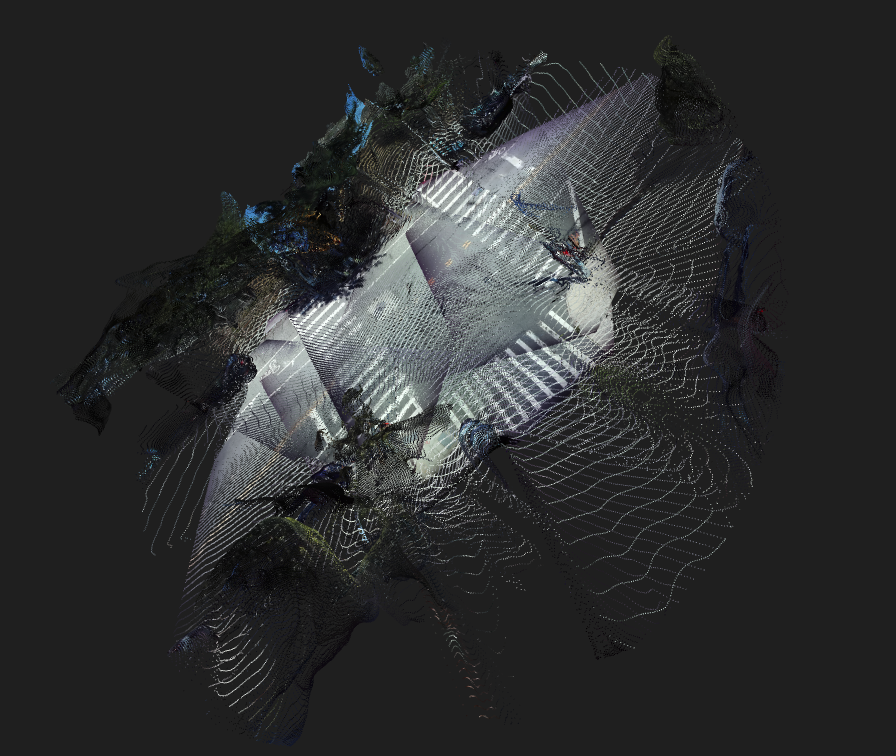
\includegraphics[width=0.8\linewidth]{assets/Dust3r_pointcloud.png}
    \caption{DUSt3R 3D point cloud}
    \label{fig:dust3r_pointcloud}
\end{figure}
\subsection{Pass 2: Dynamic Object Tracking}
\subsubsection{\green{Per-Camera Detection and Tracking}}
\green{For each camera independently, we apply YOLOv8x~\cite{yolov8} for object detection on pedestrian and vehicle classes. ByteTrack~\cite{bytetrack} maintains object identities across frames by associating detection boxes, including low-confidence detections to handle occlusions. For each track, we project the 2D bounding box bottom center to a 3D ground-contact point using camera parameters from Pass 1 and a RANSAC-fitted ground plane from the static point cloud. We accumulate 3D positions over time to create 3D trails and classify each track as stationary or moving based on 3D displacement thresholds and 2D motion variance. This produces per-camera motion summaries with track metadata and annotated visualization videos for all 8 cameras.}
\begin{figure}[h!]
    \centering
    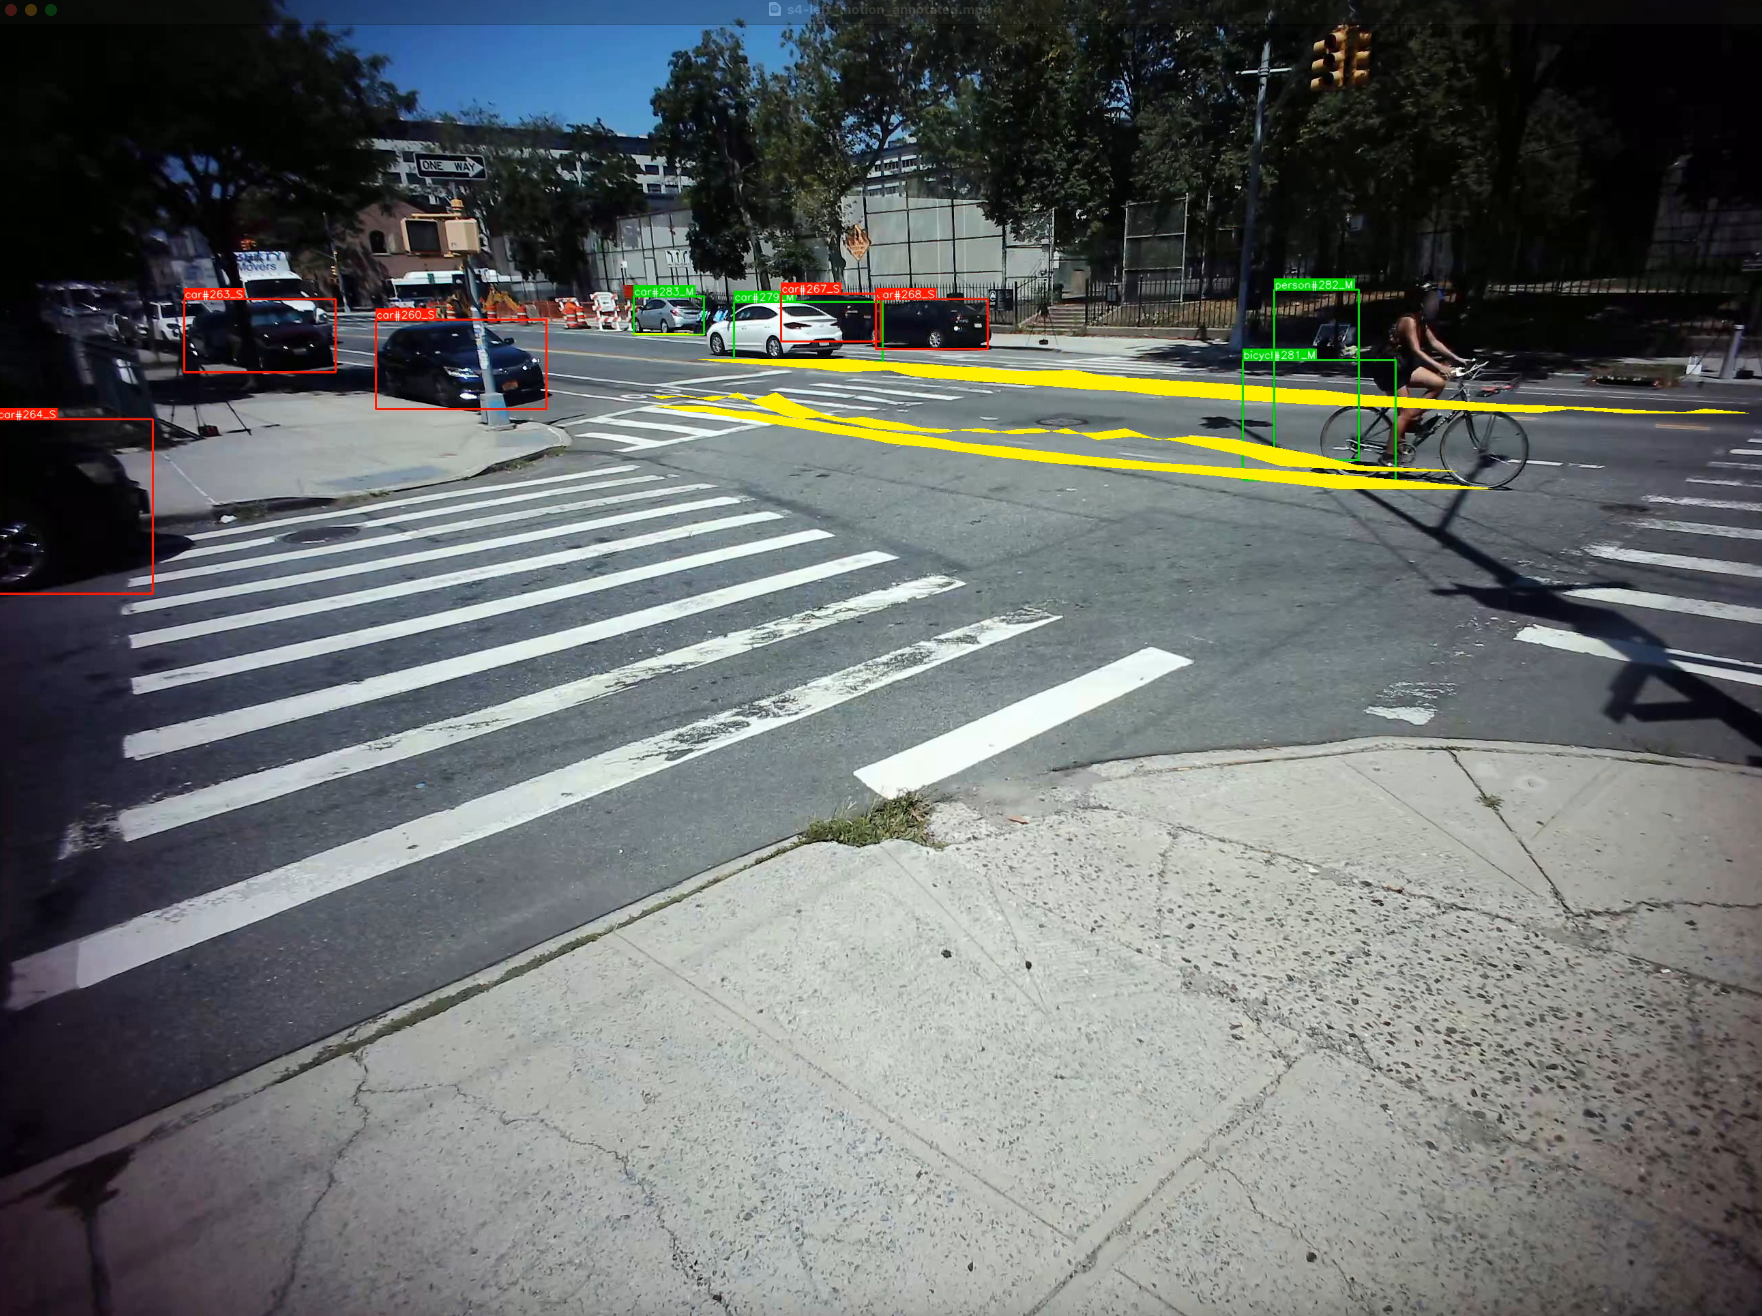
\includegraphics[width=0.8\linewidth]{assets/object_tracking.png}
    \caption{Object tracking per camera}
    \label{fig:object_tracking}
\end{figure}
\subsubsection{\red{Multi-Camera Association}}
\red{To merge tracks across cameras viewing the same object, we will aggregate all per-camera tracks and perform multi-camera association using union-find clustering. Two tracks will be merged if they satisfy: (1) same category (person/vehicle), (2) 3D spatial proximity ($\leq$2.0m for vehicles, $\leq$1.0m for persons), and (3) temporal overlap ($\geq$0.3s absolute and $\geq$30\% relative). Each cluster will represent one global object instance with a unique ID across all camera views.}
\subsubsection{\red{Canonical Primitive Representation}}
\red{Each global object is represented as a canonical 3D primitive in the DUSt3R world frame.}

\red{\textbf{Vehicles:} Unlike standard axis-aligned bounding boxes (AABB) which significantly overestimate volume during turns, we utilize Motion-Oriented Bounding Boxes (OBB). We initialize a canonical box centered at the track position and rotate it to align with the track's smoothed 3D velocity vector. This ensures the primitive fits the vehicle's actual heading, preventing false occlusion detection at intersection corners. Class-specific dimensions are used (e.g., car: 4.5$\times$1.8$\times$1.5m, truck: 8.0$\times$2.5$\times$3.0m).}

\red{\textbf{Pedestrians:} Represented as vertical cylinders (radius 0.4m, height 1.7m) centered at the track coordinate.}

\red{Centers are computed as the mean of member track 3D positions. This representation enables efficient ray-geometry intersection testing for LoS analysis.}

\subsection{\red{Pass 3: Line-of-Sight Audit}}
\red{For visibility analysis, we implement a ray-casting pipeline that determines precisely when an approaching vehicle becomes visible to a pedestrian. To handle the complexity of dense point clouds and arbitrary metric scales, we employ spatial voxelization and biological scale calibration.}

\subsubsection{\red{Scale Calibration and Spatial Indexing}}
\red{Since DUSt3R outputs geometry in arbitrary units, we recover metric scale using a biological prior. We calculate the median height of high-confidence pedestrian tracks in the unscaled space and compute a scale factor $S$ to anchor this median to 1.7m (average human height). This aligns the entire scene to real-world dimensions without relying on potentially degraded road markings.}

\red{To make ray-casting computationally feasible against a dense point cloud (15k points/m$^2$), we downsample the static scene into a Voxel Grid (20cm leaf size). This creates a lightweight occupancy map that preserves major occluders (poles, parked trucks) while significantly accelerating intersection testing.}

\subsubsection{\red{Visibility Scoring}}
\red{We define visibility not as a binary state, but as a confidence score. For each pedestrian-vehicle pair:}

\begin{enumerate}
    \item \red{\textbf{Ray Bundle Casting:} We cast rays from the pedestrian's eye point (1.6m height) to $K=5$ keypoints on the vehicle (bumper center, headlights, hood, roof).}
    \item \red{\textbf{Visibility Score ($V_t$):} A vehicle is classified as \textit{Visible} only if $>60\%$ of rays reach the target without intersecting occupied voxels or other dynamic primitives.}
    \item \red{\textbf{Occluder Identification:} For each blocked ray, we identify whether the occlusion is caused by static infrastructure (poles, signs), parked vehicles, or moving vehicles, enabling targeted safety recommendations.}
\end{enumerate}